%==============================================================================
\documentclass[11pt,oneside,onecolumn,letterpaper]{article}
\usepackage{times}
\usepackage[paperwidth=8.5in, paperheight=11in,
top=2.5cm, bottom=2.6cm, left=2.58cm, right=2.53cm]{geometry}
%\setlength{\textheight} {9.00in}
%\setlength{\textwidth}  {6.40in}
%\setlength{\topmargin}  {-0.50in}
%%\setlength{\headheight} {0.00in}
%%\setlength{\headsep}     {0.40in}
%\setlength{\oddsidemargin}{-0.010in}
%\setlength{\evensidemargin}{-0.00in}
%==============================================================================
%\usepackage{algorithm}
\usepackage{amssymb}
\usepackage{color,soul}
\usepackage{booktabs}
\usepackage{graphicx}
\usepackage{latexsym}
\usepackage{subfigure}
\usepackage{wrapfig}
\usepackage{amsmath}
\usepackage{amsthm}
\usepackage[hyphens]{url}
\usepackage{pifont}
\usepackage{xcolor}
\usepackage{colortbl}
\usepackage{indentfirst}
\usepackage[lined, boxed, linesnumbered]{algorithm2e}
\usepackage[square, comma, sort&compress, numbers]{natbib}

\newcounter{alg}
\newenvironment{enum-ref}{
	\begin{list}%
		{[\arabic{alg}]} {\usecounter{alg}
			\setlength{\leftmargin} {0.25in}
			\setlength{\labelwidth} {0.30in}
			\setlength{\rightmargin}{0.00in}
			\setlength{\topsep}     {0.00in}}
	}{\end{list}}

\newenvironment{enum-number}{
	\begin{list}%
		{\arabic{alg})} {\usecounter{alg}
			\setlength{\leftmargin} {0.25in}
			\setlength{\labelwidth} {0.30in}
			\setlength{\rightmargin}{0.00in}
			\setlength{\topsep}     {0.00in}}
	}{\end{list}}

\newenvironment{enum-nonum}{
	\begin{list}%
		{$\bullet$} {
			\setlength{\leftmargin} {0.25in}
			\setlength{\labelwidth} {0.30in}
			\setlength{\rightmargin}{0.00in}
			\setlength{\topsep}     {0.00in}}
	}{\end{list}}

\newcommand{\ziming}[1]{%
	\begingroup
	\definecolor{hlcolor}{RGB}{20, 255, 20}\sethlcolor{hlcolor}%
	\textcolor{black}{\hl{\textit{\textbf{Ziming:} #1}}}%
	\endgroup
}

\let\chapter\section

%==============================================================================
\pagestyle{plain}
%==============================================================================

\title{Medical Infrastructure Supply Chain (MISC) \\ System Design}
\author{MITRE eCTF 2024\\Team \textbf{Cacti}\\ University at Buffalo}
\date{}



\begin{document}
	%%
	%=============================================================================
	\normalsize
	
	
	\maketitle
	%\date{}
	
	\renewcommand{\thepage}{System Design, Team Cacti, University at Buffalo--\arabic{page}}
	\setcounter{page}{1} \normalsize
	%
	%\renewcommand{\baselinestretch}{1.2}
	%\normalsize
	%\vspace{0.1in}
	%\centerline{\textbf{\Large }}
	%\renewcommand{\baselinestretch}{1.0}
	%\normalsize
	
	\newcommand{\flagRollback}{\textsf{Rollback}\xspace}
	
	\section{Introduction}
	The Medical Infrastructure Supply Chain (MISC) system simulates a supply chain security solution for microcontrollers on a medical device.
	Our design consists of three parts: host computer, Application Processor (AP), and Component (CP).
	The MISC system includes one AP and two CPs connected via an I2C bus.
	The host computer is a general-purpose computer communicating with the AP over a serial interface.
	The host tools in the host computer send commands to and receive messages from the AP.
	
	The following summarizes the features of the MISC system:
	\begin{itemize}
		\item The AP can list provisioned and presented CP IDs.
		\item The whole system will only boot up when all the provisioned CPs are present and valid.
		\item The AP can retrieve attestation data from a CP with the correct PIN code.
		\item After replacing a CP,
		the AP needs to be notified of the change of a provisioned CP ID.
		\item The integrity and authenticity of communication messages between AP and CP are protected.
	\end{itemize}
	
	\section{Security Requirements}
	
	This section defines the security requirements of our design.
	
	The AP and CPs must be \textit{valid} (built by the organizers) for the MISC system to work properly.
	
	In the sections below,
	the term \textit{nonce} refers to a random number,
	which is mainly used for a challenge in the challenge-response mechanism.
	
	The term \textit{purpose label} is a 1-byte number that marks the purpose of the message,
	for example,
	different numbers for booting,
	communicating,
	attesting,
	sending,
	and reading.
	
	\subsection{SR1 \& SR2}
	\textbf{The Application Processor (AP) should only boot if all expected CPs are present and valid.}
	
	\textbf{CPs should only boot after being commanded to by a valid AP that has confirmed the integrity of the device.}
	
	\paragraph{How we address it:}
	The AP needs to verify all the present CPs have provisioned IDs and that they are valid CPs built by the organizers.
	We use the public-key cryptography algorithm and challenge-response authentication.
	There are two key pairs,
	the AP holds the first private key and the second public key,
	while the CP holds the first public key and the second private key.
	
	When the host computer sends the boot command to the AP,
	the AP sends the boot command and a generated nonce (challenge) to the CP.
	The CP makes up a response by signing the booting purpose label,
	nonce,
	and CP ID with the second private key.
	Then,
	it generates another nonce and replies the response and the new nonce to the AP.
	The AP verifies the reply with the second public key.
	The booting purpose label,
	nonce,
	and CP ID should be correct.
	After receiving the replies from all the provisioned CPs,
	the AP makes up the responses for each CP using the same signing method mentioned before with the first private key.
	For a CP,
	it will verify the response from the AP using the first public key and boot up if verification passes.
	
	The boot messages will be stored as encrypted text in both AP and CP.
	When a CP boots,
	it sends the encrypted boot message to AP,
	and AP decrypts it.
	When the AP boots,
	it retrieve and decrypts the boot message.
	
	The signing process includes the purpose label and CP ID to mitigate response reuse attacks (from other functionalities or other CPs).
	
	\subsection{SR3}
	\textbf{The Attestation PIN and Replacement Token should be kept confidential.}
	\paragraph{How we address it:}
	The Attestation PIN and Replacement Token will not be stored in plain text or hardcoded in the program (e.g., use the macro generated in the building phase).
	The PIN and the Token will be hashed using a keyed-hash algorithm during the building process,
	and the PIN and Replacement Token macros will be replaced with the two hash strings.
	AP holds the hash key.
	After receiving a PIN or a token,
	the AP will apply the keyed hash to the input,
	and compare the hash string with the saved one.
	The comparison time is constant regardless of the content of the PIN or Replacement Token to mitigate a timing side-channel attack.
	To mitigate a brute force attack,
	the AP will delay 4 seconds after receiving a wrong PIN or token.
	
	\subsection{SR4}
	\textbf{CP Attestation Data should be kept confidential.}
	\paragraph{How we address it:}
	Use symmetric encryption to encrypt the CP Attestation Data with a Python script to replace the plain text with the encrypted text in macros when building a CP.
	The key is generated based on a shared secret between AP and CP.
	A CP does not have the decryption functionality during runtime.
	When requesting the attestation data,
	a CP puts the encrypted text in the I2C buffer.
	The AP reads the encrypted text,
	decrypts it,
	and sends it to the host computer.
	
	A CP needs to verify if the Attestation Data reading request message is from the valid AP.
	public-key cryptography algorithm and challenge-response mechanism are used for the verification process.
	The AP holds the private key,
	and the CP holds the public key.
	The AP sends a request message to the CP
	The CP generates a nonce and sends it to the AP as the challenge.
	The AP signs attesting purpose label,
	the challenge,
	and the CP ID using the private key and sends it back to the CP as the response.
	The CP verifies the response using the public key and checks if the purpose label,
	challenge,
	and CP ID are correct.
	
	The signing process includes the purpose label and CP ID to mitigate response reuse attacks (from other functionalities or other CPs).
	
	\subsection{SR5}
	\textbf{The integrity and authenticity of messages sent and received using the post-boot MISC secure communications functionality should be ensured.}
	\paragraph{How we address it:}
	With the public-key cryptography algorithm,
	we use the challenge-response authentication for message authenticity and digital signature for message integrity.
	There are two key pairs,
	the AP holds the first private key and the second public key,
	the CP holds the first public key and the second private key.
	
	To send a message to a CP,
	the AP sends the sending message command to the CP.
	The CP generates a nonce as the challenge for the AP,
	and the AP signs the reading purpose label,
	nonce,
	and CP ID using the first private key as the response.
	The AP also signs the message with the same key.
	The AP sends the response,
	message,
	and the message signature to the CP.
	The CP verifies the response and the message signature by using the first public key.
	It receives the message if validations pass.
	
	To read a message from a CP,
	the AP sends the reading command and a nonce challenge to the CP.
	The CP signs the challenge with the second private key as the response,
	and puts the response,
	message,
	and the signature of the message (with the second private key) to the I2C buffer waiting for the AP to read.
	The AP reads the response,
	message,
	and the signature.
	It verifies the response and the message signature using the second public key.
	
	The signing process includes the purpose label and CP ID to mitigate response reuse attacks (from other functionalities or other CPs).
	
	
	\section{Security Implementations}
	
	
	\subsection{Build MISC System}
	\subsubsection{Build Deployment}
	Attackers will NEVER be given access to the Deployment Secrets generated in this step.
	\begin{figure}[h]
		\centering
		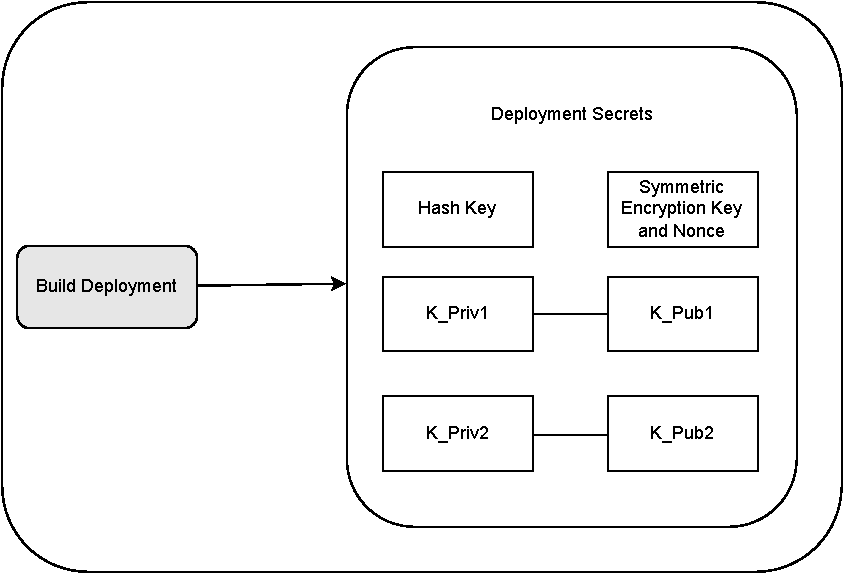
\includegraphics[width=0.65\textwidth]{pics/secret.pdf}
		\caption{Deployment Secret}
		\label{fig:secret}
	\end{figure}
	
	Figure \ref{fig:secret} shows the Deployment Secrets.
	During the building deployment process,
	a hash key (keyed-hash algorithm for PIN and replace token),
	a symmetric encryption key (for encrypting the attestation data),
	and two pairs of public and private keys will be generated.
	The hash key and symmetric encryption key (containing salt and nonce) will be shared among the AP and all the CPs.
	AP will store the first private key of \texttt{K\_Pri1} and the second public key of \texttt{K\_Pub2}.
	CP will store the second private key of \texttt{K\_Pri2} and the first public key of \texttt{K\_Pub1}.
	We generate the Deployment Secrets randomly when building deployment to prevent the attacker from retrieving it through the source code.
	
	\subsubsection{Build AP and CP Firmware}
	To build the AP firmware,
	the number of provisioned CPs,
	provisioned CP IDs,
	attestation PIN code,
	and replace Token need to be provided.
	The AP firmware contains \texttt{K\_Pri1},
	\texttt{K\_Pub2},
	Argon2 hash key and salt,
	AEAD key and nonce,
	hashed PIN,
	and hashed replaced token.
	
	
	To build the CP firmware,
	the CP ID and attestation data need to be provided.
	The attestation data includes location,
	date,
	and customer name.
	The CP firmware contains \texttt{K\_Pri2},
	\texttt{K\_Pub1},
	and cipher text of attestation data.
	
	\subsection{Load Devices and Booting}
	\subsubsection{Load AP and CP Firmware}
	The firmware will be loaded by the provided host tool,
	teams are not allowed to modify this step.
	
	\subsubsection{First Booting}
	Devices will be initialized at the first boot.
	The AP will store provisioned CP IDs in plain text,
	the \texttt{K\_Pri1} key,
	\texttt{K\_Pub2} key,
	hash key,
	and symmetric key in the flash memory.
	The CP stores the \texttt{K\_Pri2} and \texttt{K\_Pub1} keys.
	
	\subsection{Functionalities}
	The term \textit{packet} refers to all the communication data either the AP sends to a CP,
	or the AP reads from a CP.
	
	The I2C address of a CP derives from the CP ID.
	
	A timeout (usually less than 0.2 seconds) is applied for I2C communications involving a response (e.g., challenge-response or sending a request package and waiting for a response package).
	After the timeout,
	the sender will terminate the current functionality. (e.g., attest, boot, ...)
	
	\subsubsection{Listing}
	The Listing functionality checks the provisioned CP IDs in the AP and the IDs of all the presented CPs.
	As CP IDs are not secrets,
	there is nothing to protect during this process.
	
	\begin{figure}[h]
		\centering
		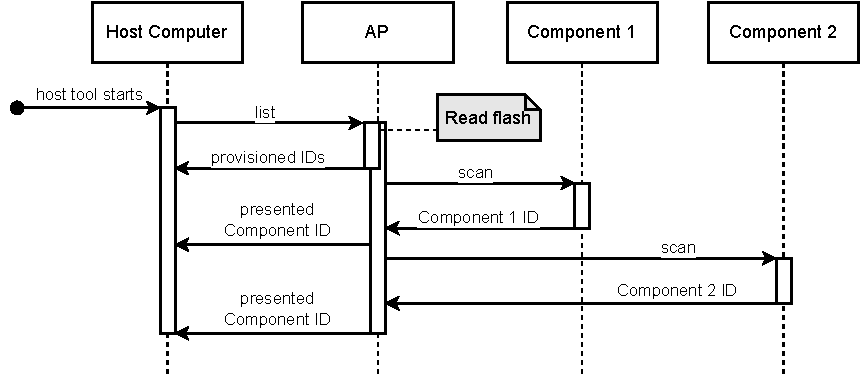
\includegraphics[width=0.8\textwidth]{pics/list.pdf}
		\caption{Listing Sequence}
		\label{fig:functionality_list}
	\end{figure}
	
	The process (shown in Figure \ref{fig:functionality_list}) is described as follow:
	
	\begin{enumerate}
		\item The host computer sends the \texttt{list} command through USB to the AP.
		\item The AP reads all the provisioned CP IDs from its flash memory and sends the IDs back to the host computer.
		\item The AP sends the \texttt{scan} command to all the possible CP IDs one by one over the I2C bus.
		\item For one specific ID,
		if the CP with this ID is presented,
		the CP puts the ID value in the I2C buffer for the AP to read.
		\item The AP reads the ID value from this CP and sends the ID value to the host computer as one present CP ID.
		
	\end{enumerate}
	
	\subsubsection{Boot}
	This functionality requires the AP to test if all the provisioned CPs are present and valid before the AP boots.
	The AP sends commands to all the CPs to let them boot,
	and the CPs must ensure that the boot command is from the valid AP before booting.
	
	\begin{figure}[h]
		\centering
		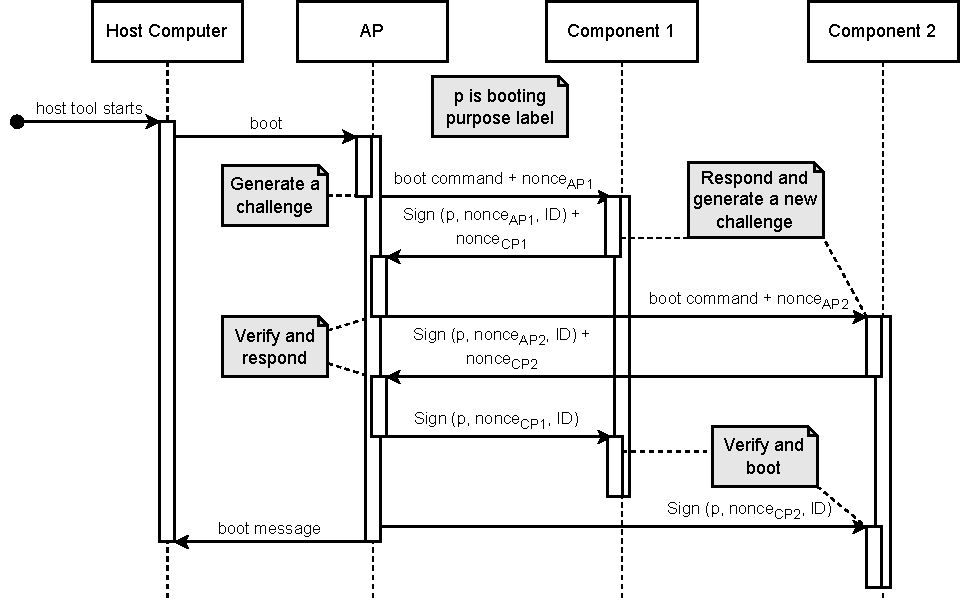
\includegraphics[width=0.8\textwidth]{pics/boot.pdf}
		\caption{Boot Sequence}
		\label{fig:functionality_boot}
	\end{figure}
	
	The process (shown in Figure \ref{fig:functionality_boot}) is described as follow:
	\begin{enumerate}
		\item The host computer sends the \texttt{boot} command to the AP.
		\item The AP checks all the provisioned CPs one by one to make sure they are present and valid.
		\item For each provisioned CP,
		the AP generates a nonce as the challenge.
		It then sends the \texttt{boot} command,
		challenge,
		and the corresponding CP ID.
		\item After receiving the boot command and the challenge,
		the CP makes up the response by signing a boot purpose label,
		the challenge,
		along with the CP ID using the \texttt{K\_Pri2} key.
		It then creates a new challenge by generating a nonce and puts the response and new challenge to the I2C buffer waiting for the AP to read.
		\item The AP reads the response from the CP and verifies the response using the \texttt{K\_Pub2}.
		It checks if the purpose label is for booting,
		the nonce is the same as the originally generated one,
		and the CP ID is correct.
		The AP also records the challenge from this CP.
		\item For a validation failure,
		the AP will delay for 4 seconds to mitigate a brute force attack and terminate the booting process.
		\item If all the CPs are present,
		the AP then tries to boot them all.
		\item To boot a CP,
		the AP finds the challenge sent by this CP before.
		Then sign the booting purpose label, nonce, and CP ID with the \texttt{K\_Pri1} key as the response.
		The AP sends the response to this CP.
		\item After receiving the response from the AP,
		the CP verifies the response by using the \texttt{K\_Pub1}.
		The CP will boot up if verification passes.
		\item The CP retrieves and sends encrypted CP boot message to AP, and AP decrypts it and sends to the host computer.
		\item The AP retrieve and decrypts the AP boot message and send to the host computer.
	\end{enumerate}
	
	\subsubsection{Replace}
	The Replace functionality is for replacing a CP on the medical device.
	The technician in a repair station needs to tell the AP which CP ID is no longer provisioned and what the new CP ID with supplying the correct replacement Token.
	The replace Token will be hashed before comparing with the saved Token hash value.
	
	\begin{figure}[h]
		\centering
		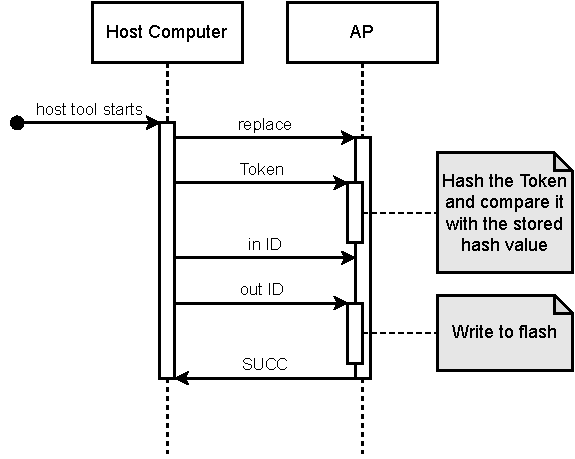
\includegraphics[width=0.55\textwidth]{pics/replace.pdf}
		\caption{Replace Sequence}
		\label{fig:functionality_replace}
	\end{figure}
	
	The process (shown in Figure \ref{fig:functionality_replace}) is described as follow:
	
	\begin{enumerate}
		\item The host computer sends the \texttt{replace} command to the AP.
		\item The AP enters the \texttt{replace} mode and waits for the host computer to send the replace Token.
		\item After receiving the Token,
		the AP applies the keyed-hash algorithm to the Token and compares it with the stored hash value.
		All the characters in the hash value are compared one by one.
		The comparison time is always constant no matter if the received Token is correct or not.
		If a wrong Token is received,
		the AP will randomly delay for 4 seconds to mitigate brute force and then terminate the replace mode.
		For a correct Token received,
		the AP will wait for the host computer to send the old (currently provisioned) and new IDs.
		\item The AP modifies the flash memory after receiving the two IDs and sends a success message to the host computer.
		And the new ID becomes the provisioned ID.
		The AP stores the new ID in the flash memory.
	\end{enumerate}
	
	\subsubsection{Attestation}
	The functionality is for getting the attestation data from one specific CP by supplying the correct PIN code and the CP ID.
	The attestation data is encrypted in the flash memory,
	so decrypting is necessary after retrieving the data.
	Also,
	the PIN code will be hashed before comparing with the saved PIN code hash value.
	
	\begin{figure}[h]
		\centering
		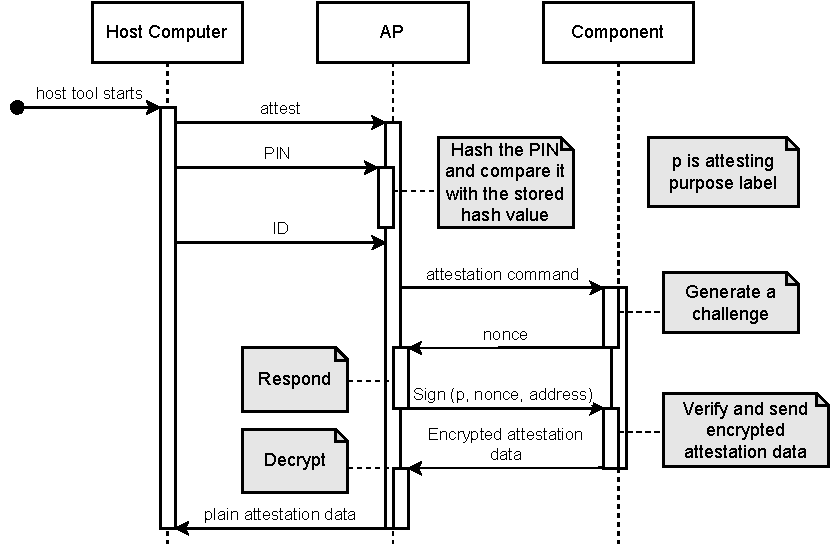
\includegraphics[width=0.8\textwidth]{pics/attest.pdf}
		\caption{Attestation Sequence}
		\label{fig:functionality_attest}
	\end{figure}
	
	The process (shown in Figure \ref{fig:functionality_attest}) is described as follow:
	\begin{enumerate}
		\item The host computer sends the \texttt{attest} command to the AP
		\item The AP enters the \texttt{attestation} mode and waits for the host computer to send the PIN code
		\item After receiving the PIN code,
		the AP applies the keyed-hash algorithm to the PIN and compares it with the stored one.
		The comparison time is always constant no matter the correctness of the PIN.
		The AP will randomly delay for 4 seconds to mitigate brute force and then terminate the attestation mode for a wrong PIN.
		When given a correct PIN,
		the AP tries to acquire the attestation data from the specific CP with the ID given by the host computer.
		\item The AP sends the \texttt{attestation} command to the CP.
		\item The CP generates a nonce and sends it as a challenge to the AP.
		\item The AP signs the attesting purpose label,
		nonce,
		and the CP ID using the \texttt{K\_Pri1} key and sending it as the response back to the CP.
		\item The CP verifies the response with the \texttt{K\_Pub1} key to check if the attesting purpose label,
		nonce,
		and the ID is correct.
		If validation fails,
		the CP sends the verification failure message to the AP,
		and the AP randomly delays for 4 seconds to prevent brute force and terminate the attestation mode.
		Otherwise,
		the CP puts the encrypted attestation data in the I2C buffer waiting for the AP to read.
		\item The AP decrypts the data using the symmetric algorithm and sends the plain attestation data to the host computer.
	\end{enumerate}
	
	\subsubsection{POST-BOOT Communication}
	After the AP and CPs boot up,
	the communication between the AP and a CP is through the I2C bus.
	The AP is the master device,
	while the CPs are slave devices.
	Thus,
	the AP can send messages to or read messages from a CP.
	However, the CP cannot send messages directly to the AP in normal situations.
	The integrity and authenticity of the communication are necessary.
	
	\begin{figure}[h]
		\centering
		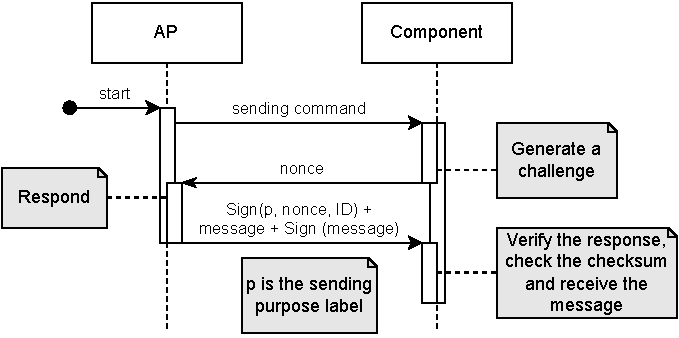
\includegraphics[width=0.7\textwidth]{pics/post1.pdf}
		\caption{Sending Message Protocol Sequence}
		\label{fig:functionality_post1}
	\end{figure}
	
	The sending message process is shown in Figure \ref{fig:functionality_post1}.
	\begin{enumerate}
		\item The AP sends the \texttt{sending} command to one specific CP.
		\item The CP generates a nonce as the challenge for the AP.
		\item The AP signs the sending purpose label,
		nonce,
		and the CP I2C address using the \texttt{K\_Pri1} key as the response for the CP.
		The AP sends the response,
		a signature of the message (signed using the \texttt{K\_Pri1} key),
		and message to the CP.
		\item The CP verifies using the \texttt{K\_Pub1} key the response by checking if the reading purpose label,
		nonce,
		and the address is correct to ensure authenticity.
		\item The CP then verifies the message signature by using the \texttt{K\_Pub1} key to ensure the message integrity.
		\item If the two verifications pass,
		the CP receives the message.
	\end{enumerate}
	
	\begin{figure}[h]
		\centering
		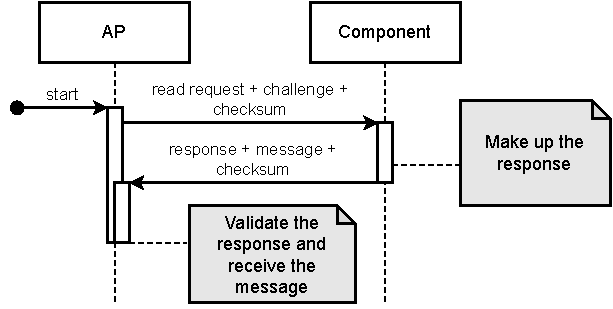
\includegraphics[width=0.7\textwidth]{pics/post2.pdf}
		\caption{Reading Message Protocol Sequence}
		\label{fig:functionality_post2}
	\end{figure}
	
	The reading message process is shown in Figure \ref{fig:functionality_post2}.
	\begin{enumerate}
		\item The AP sends the \texttt{reading} command and a generated nonce to one specific CP.
		\item The CP signs the reading purpose label,
		nonce,
		and the address with the \texttt{K\_Pri2} key as the response.
		It puts the response,
		a signature of the message signed using the \texttt{K\_Pri2} key,
		and message in the I2C buffer,
		waiting for the AP to read.
		\item The AP reads the packet from the CP.
		\item The AP verifies the response using the \texttt{K\_Pub2} key and checks if the reading purpose label,
		nonce,
		and the CP I2C address are correct.
		It then verifies the message signature by using the \texttt{K\_Pub2} to ensure the message integrity.
		If verifications pass,
		the AP accepts the message.
	\end{enumerate}
	
\end{document}
%==============================================================================
